\section{Resultados y Análisis}

En este capitulo se describen ciertos pasos y funcionamientos de la solución en general. En la figura \ref{fig:iot} esta el esquema del sistema IoT.\\

\begin{figure}[!t]
	\centering
	\caption{Esquema Solución SmartHouse [Imagen Propia]}
	\label{fig:iot}
	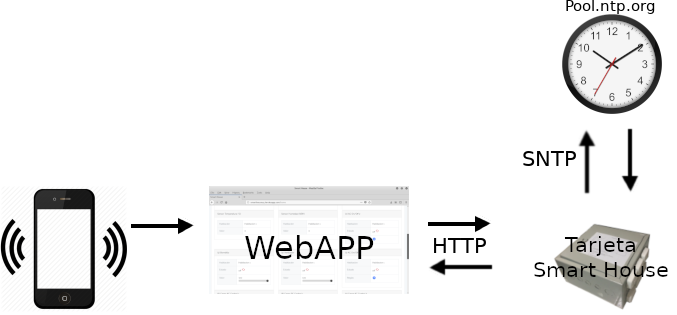
\includegraphics[width=0.8\linewidth]{Imagenes/IOT}
\end{figure}

\subsection{Software}

 La aplicación web se encuentra compuesta por los siguientes sitios y las diferentes interacciones basadas en las funciones básicas, crear, leer, actualizar y borrar (CRUD).\\

\begin{itemize}
	\item Parte Pública
	\item Parte Privada
	\begin{itemize}
		\item Intercambio de datos
		\item Panel de Control
		\begin{itemize}
			\item Crear
			\item Ver
			\item Editar
			\item Eliminar 
		\end{itemize}
	\end{itemize}
\end{itemize}

De acuerdo con la lista anterior, se toman en cuenta dos partes, una pública y una privada, como se observa en la figura \ref{fig:index}. En la parte pública se encuentra una vista con la información de contacto del fabricante, solicitudes de registro o productos y la cantidad de usuarios que actualmente estan registrados en la aplicación. En la parte privada se encuentra la interacción de los usuarios sea administrador, dueño de una casa o de una habitación, para controlar y observar sus datos.\\

\begin{figure}[!t]
\centering
\caption{Página de Inicio. [Imagen Propia]}
\label{fig:index}
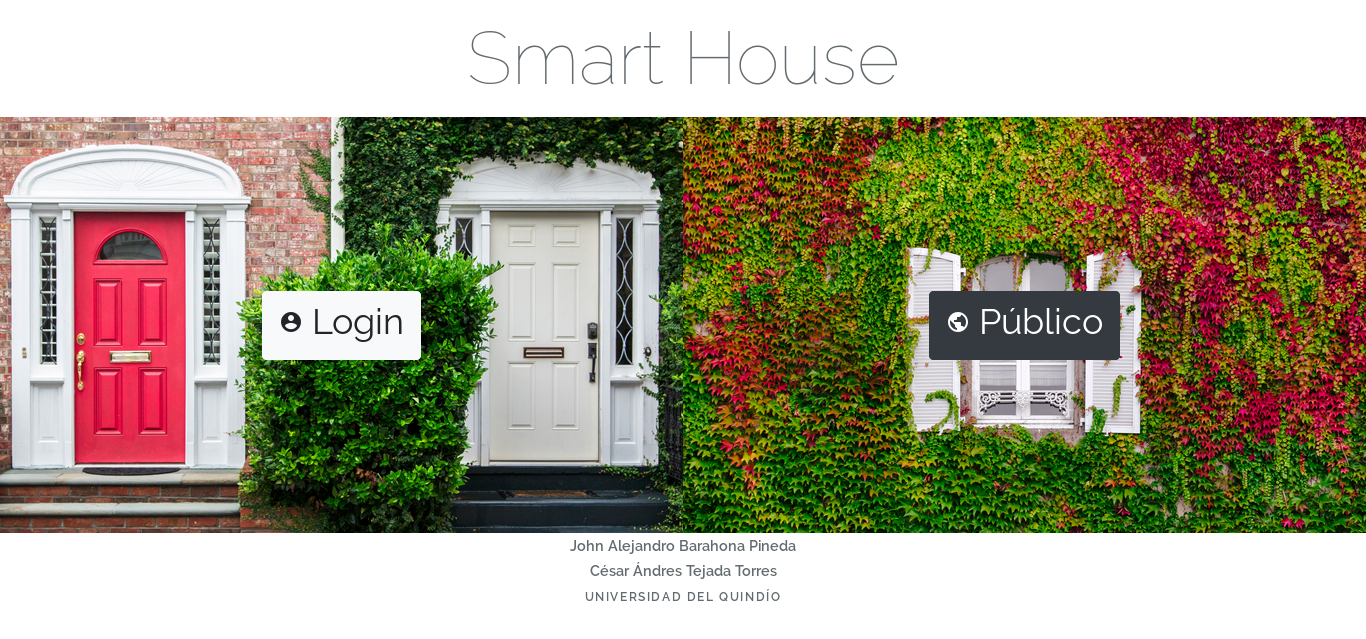
\includegraphics[width=0.9\linewidth]{Imagenes/Index}
\end{figure}

\subsubsection{Parte Pública}

En esta vista únicamente hay opciones para el contacto y solicitudes, como se menciona anteriormente, es sencilla debido a la poca información que contiene.

\subsubsection{Parte Privada}

En primera instancia, un usuario administrador tiene la posibilidad de crear, ver, editar y eliminar los registros de la aplicación, la vista de este usuario se puede observar en la figura \ref{fig:views}\textbf{(a)}. También existe el usuario dueño de la vivienda, este puede revisar y editar algunos campos de sus usuarios hijos o usuarios habitación,  en la figura \ref{fig:views}\textbf{(b)} se observa su vista. Por último, se tiene el usuario habitación que únicamente visualiza los datos  del cuarto en cuestión, según se observa en la figura \ref{fig:views}\textbf{(c)}, por tal motivo el panel de control muestra una vista general de los datos y el estado de sus dispositivos, además de tener la capacidad de editar partes básicas de su habitación y perfil.\\

Adicionalmente, si el usuario desea añadir, modificar o eliminar una regla, puede lograrlo mediante el botón de reglas en el panel de control, el cual lo redirige a una página que indica una hora de inicio y finalización en la que el bombillo led enciende y apaga respectivamente. \\

\begin{figure}[!t]
	\centering
	\caption{Vistas de Usuarios [Imagen Propia]}
	\label{fig:views}
	\subfigure[Usuario Administrador]{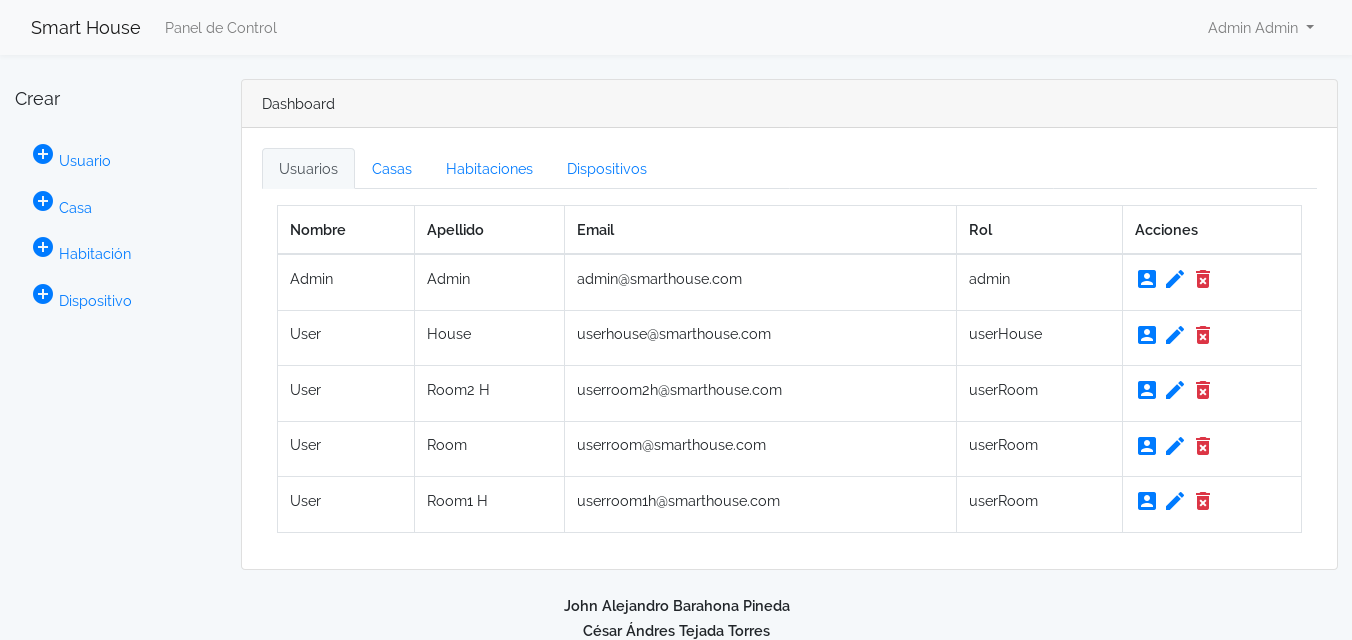
\includegraphics[width=0.9\linewidth]{Imagenes/Admin_view}}
	\subfigure[Usuario de Casa]{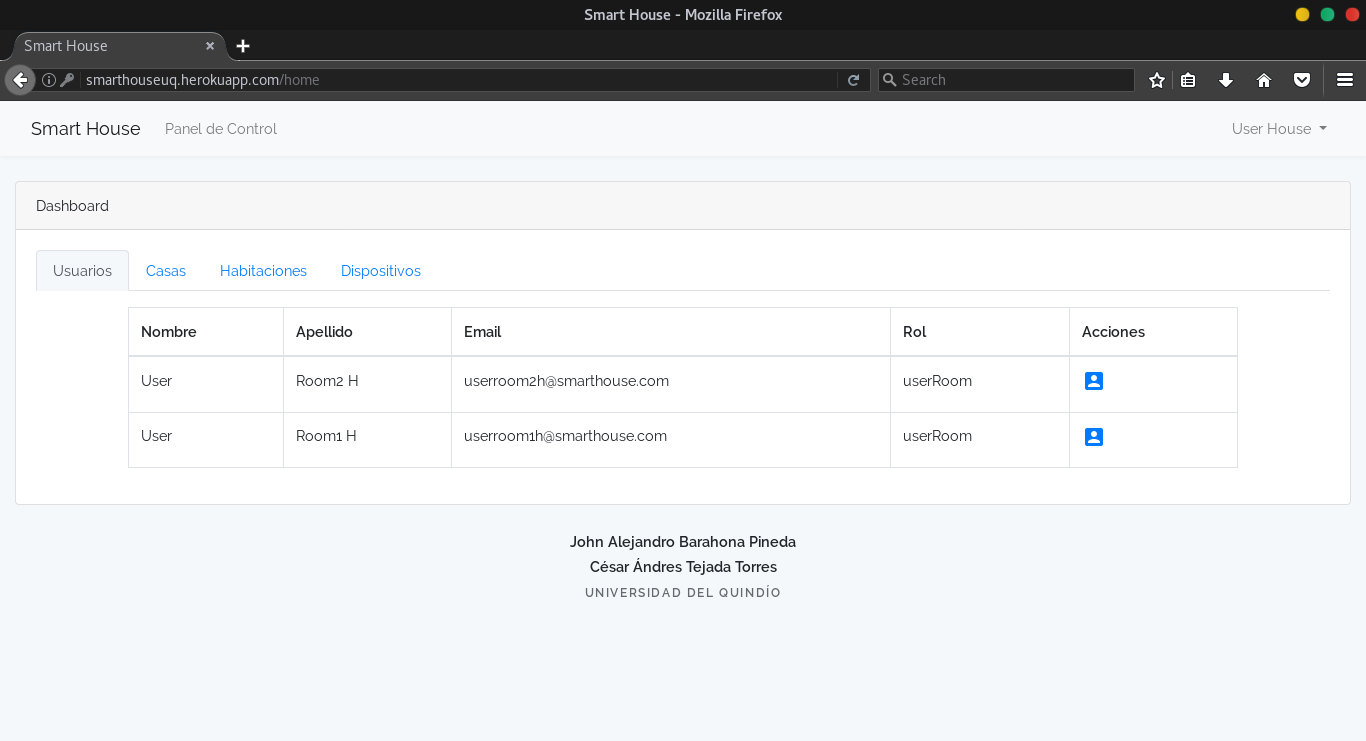
\includegraphics[width=0.45\linewidth]{Imagenes/UserH_view}}
	\subfigure[Usuario de Habitación]{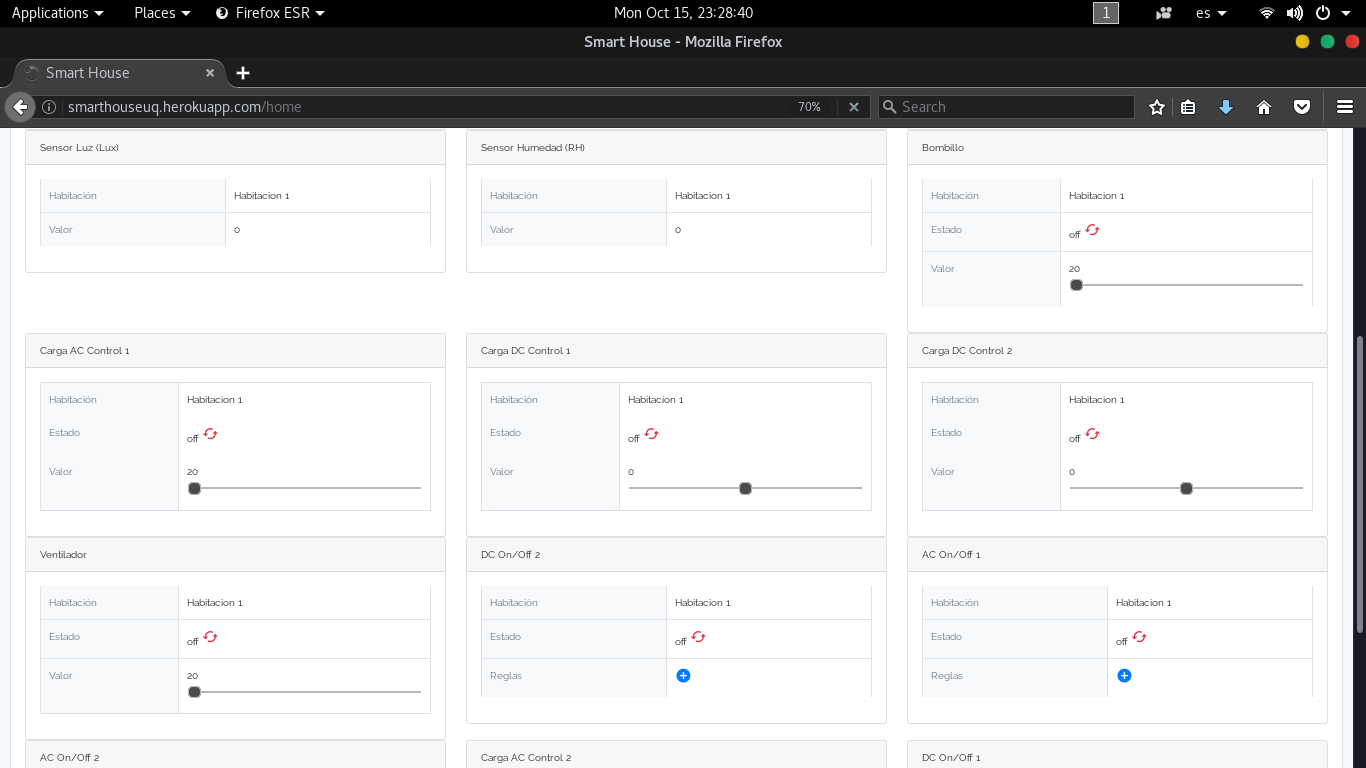
\includegraphics[width=0.45\linewidth]{Imagenes/UserR_view}}
\end{figure}

\subsubsection{Base de Datos}

La estructura de la base de datos se puede observar en la figura \ref{fig:db}, aquí se observan los diferentes campos que posee cada tabla, además de las llaves y sus relaciones, las relaciones presentes en esta estructura son de tipo 1:N, es decir, por ejemplo un usuario puede tener relacionadas N casas.\\  

\begin{figure}[!t]
\centering
\caption{Base de datos SmartHouse [Imagen Propia]}
\label{fig:db}
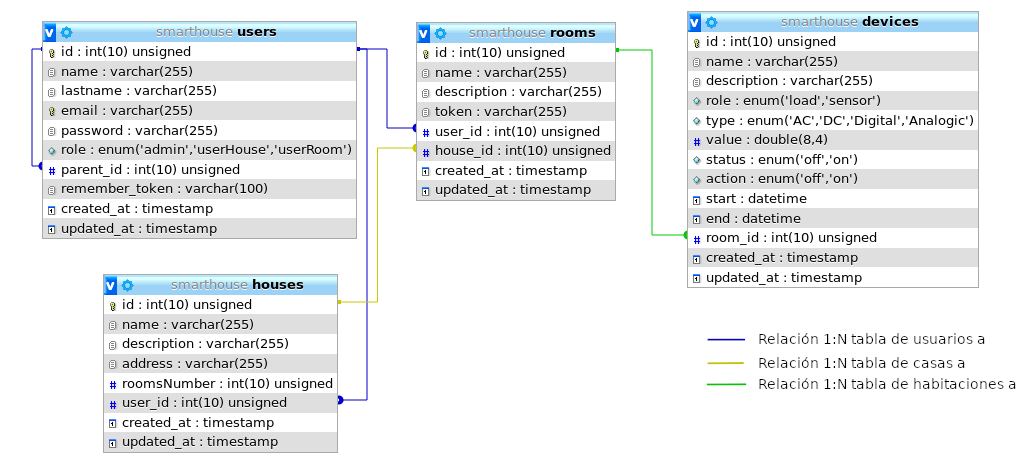
\includegraphics[width=0.8\linewidth]{Imagenes/DB}
\end{figure}

Las diversas interfaces generadas en la aplicación, permiten el monitoreo, control y la interacción del usuario con el dispositivo presente en su habitación, haciendo posible el cambio de estado de las salidas y así mismo visualizar los datos producidos por los sensores. También cabe resaltar que algunas salidas tienen la posibilidad de automatizarse a través de reglas, es decir, indicarle en que momento encender o apagar cierto dispositivo que se encuentre conectado a la tarjeta como se ha mencionado. Por otra parte, todos los datos generados de la interacción del cliente con el programa se almacenan en la base de datos enlazada a dicha aplicación permitiendo una gestión adecuada de estos. Los resultados obtenidos del diseño de este software cumplen con el objetivo a partir del cual se construye y también se tienen algunas funciones adicionales como los usuarios administradores de casa, esto asegurando la escalabilidad de la aplicación. \\

\subsection{Firmware}

El firmware se encuentra compuesto, como se ha mencionado anteriormente, de tareas, en la figura \ref{fig:tareas} se observa un bosquejo del trabajo de las diferentes tareas de las que se compone este, tomando por función principal la encargada de gestionar la conexión a Wi-Fi y almacenar sus credenciales, dependiendo del estado de si están almacenadas o no, el sistema se comporta de una u otra forma.\\

\begin{figure}[!t]
	\centering
	\caption{Esquema de Tareas [Imagen Propia]}
	\label{fig:tareas}
	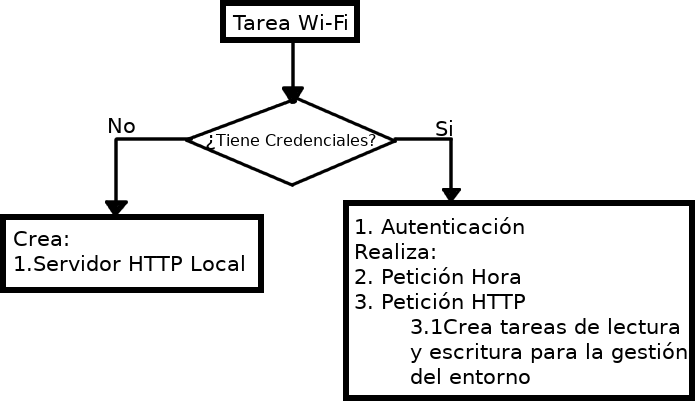
\includegraphics[width=0.8\linewidth]{Imagenes/tareas}
\end{figure}
 

\subsubsection{Escritura de Datos en la Aplicación Web}

Los datos que lee la tarjeta provienen de los diferentes sensores que tiene conectados, para la escritura de estos, en el firmware se desarrollan con varias tareas encargadas de leerlos y enviarlos a una tarea central. Los datos que están enviando contienen el id del dispositivo y la medida que lee en ese momento, estos se envían en forma de texto en formato JSON, organizándolos en la petición HTTP tipo GET; así la url que la tarjeta solicita, incluyendo el JSON de cada sensor, se observa en la figura \ref{fig:json}. La aplicación ya se encarga de almacenarlos y mostrarlos al usuario como se menciona anteriormente.\\

\begin{figure}[!t]
	\centering
	\caption{URL de la petición HTTP [Imagen Propia]}
	\label{fig:json}
	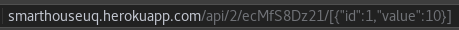
\includegraphics[width=0.9\linewidth]{Imagenes/JSON}
\end{figure}


\subsubsection{Lectura de Datos de Internet}

La tarjeta mantiene una actualización frecuente, para esto, cuando la tarjeta envía los datos de los sensores la aplicación responde con datos de cabecera HTTP, además de la información de los dispositivos que controla la tarjeta, esta los recibe en una cadena texto en formato JSON como se observa en la figura \ref{fig:httprqstesp}, los procesa y los dirige a las tareas pertinentes ya sea para encender o apagar algún dispositivo conectado a la tarjeta, también remite las reglas que el usuario ha definido.\\

\begin{figure}[!t]
	\centering
	\caption{Respues del la APP Web a la Tarjeta [Imagen Propia]}
	\label{fig:httprqstesp}
	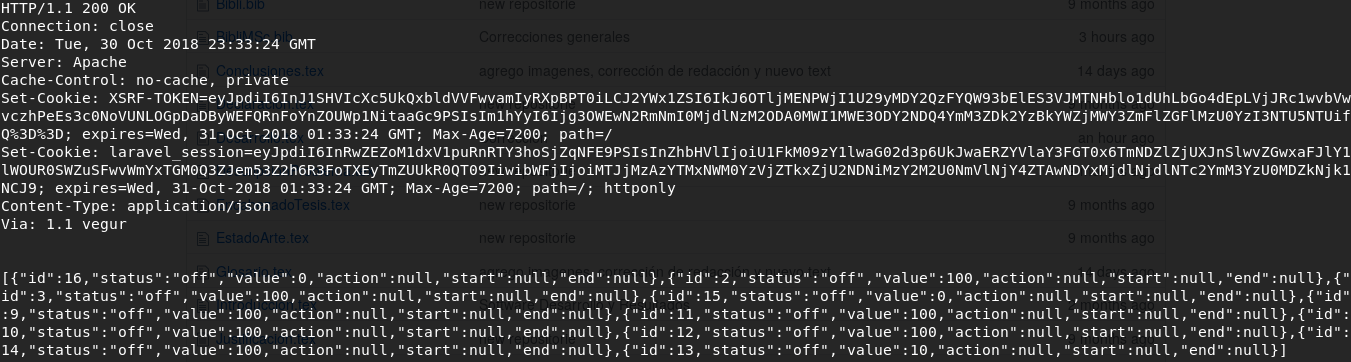
\includegraphics[width=0.9\linewidth]{Imagenes/HTTPRqstesp}
\end{figure}

Analizando los tiempos de resolución de la petición http, se tiene una media aproximada de 1s, el cual es un tiempo de respuesta aceptable dadas todas las funcionalidades provistas en el programa, aunque este tiempo varia, ya que el haber utilizado el puerto serie para observar estos resultados se agrega tiempo al procesamiento, así como también interfiere la velocidad en la conexión a internet y la señal de recepción de wi-fi.\\


\subsection{Hardware}

De acuerdo con los circuitos diseñados en la sección \ref{sec:hw}, en la figura \ref{fig:tarjeta} se observan las diferentes tarjetas ya ensambladas en una caja eléctrica para probar el funcionamiento del prototipo. Las salidas y entradas están distribuidas según lo propuesto e ilustradas en la caja eléctrica por medio de pegatinas, la figura \ref{fig:labels} muestra esta información; para las salidas AC se usan toma corrientes para conectar allí los diversos dispositivos, para las salidas DC se utilizan conectores hembra tipo banana para facilitar la conexión de estos dispositivos.\\

\begin{figure}[!t]
	\centering
	\caption{Tarjeta SmartHouse [Imagen Propia]}
	\label{fig:tarjeta}
	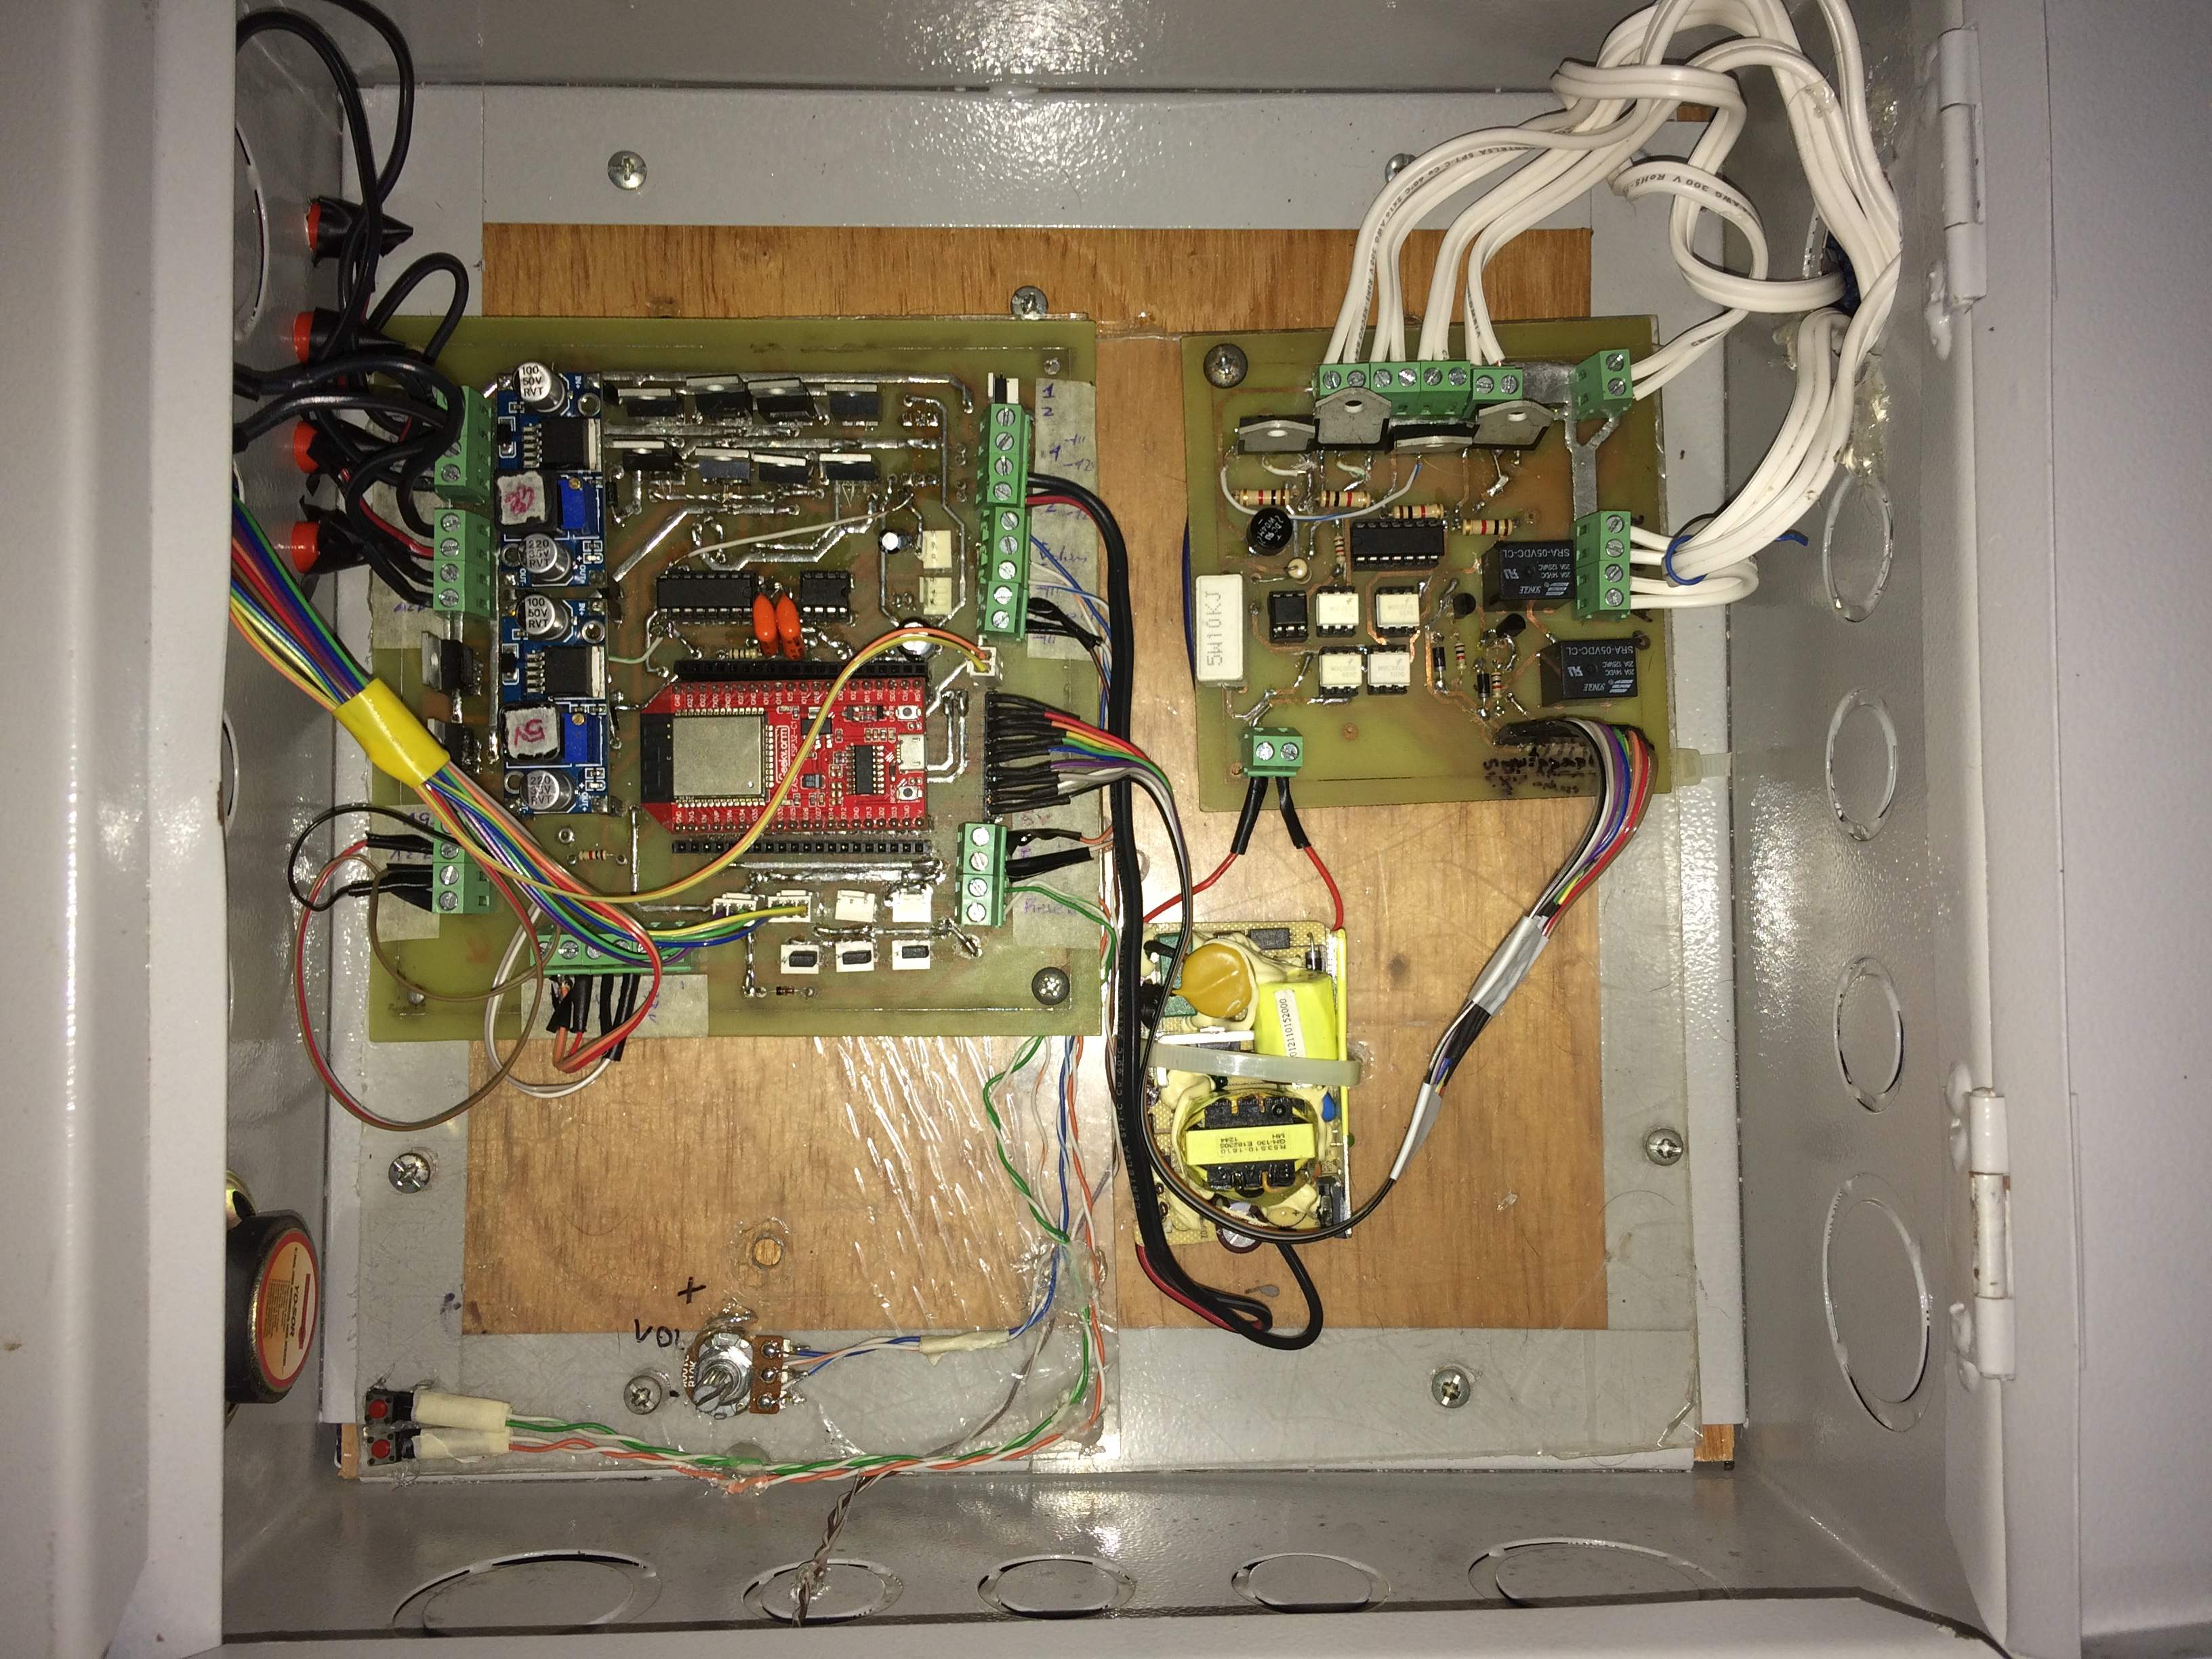
\includegraphics[width=0.6\linewidth]{Imagenes/Tarjeta}
\end{figure}

\begin{figure}[!t]
	\centering
	\caption{Descripción caja eléctrica tarjeta SmartHouse [Imagen Propia]}
	\label{fig:labels}
	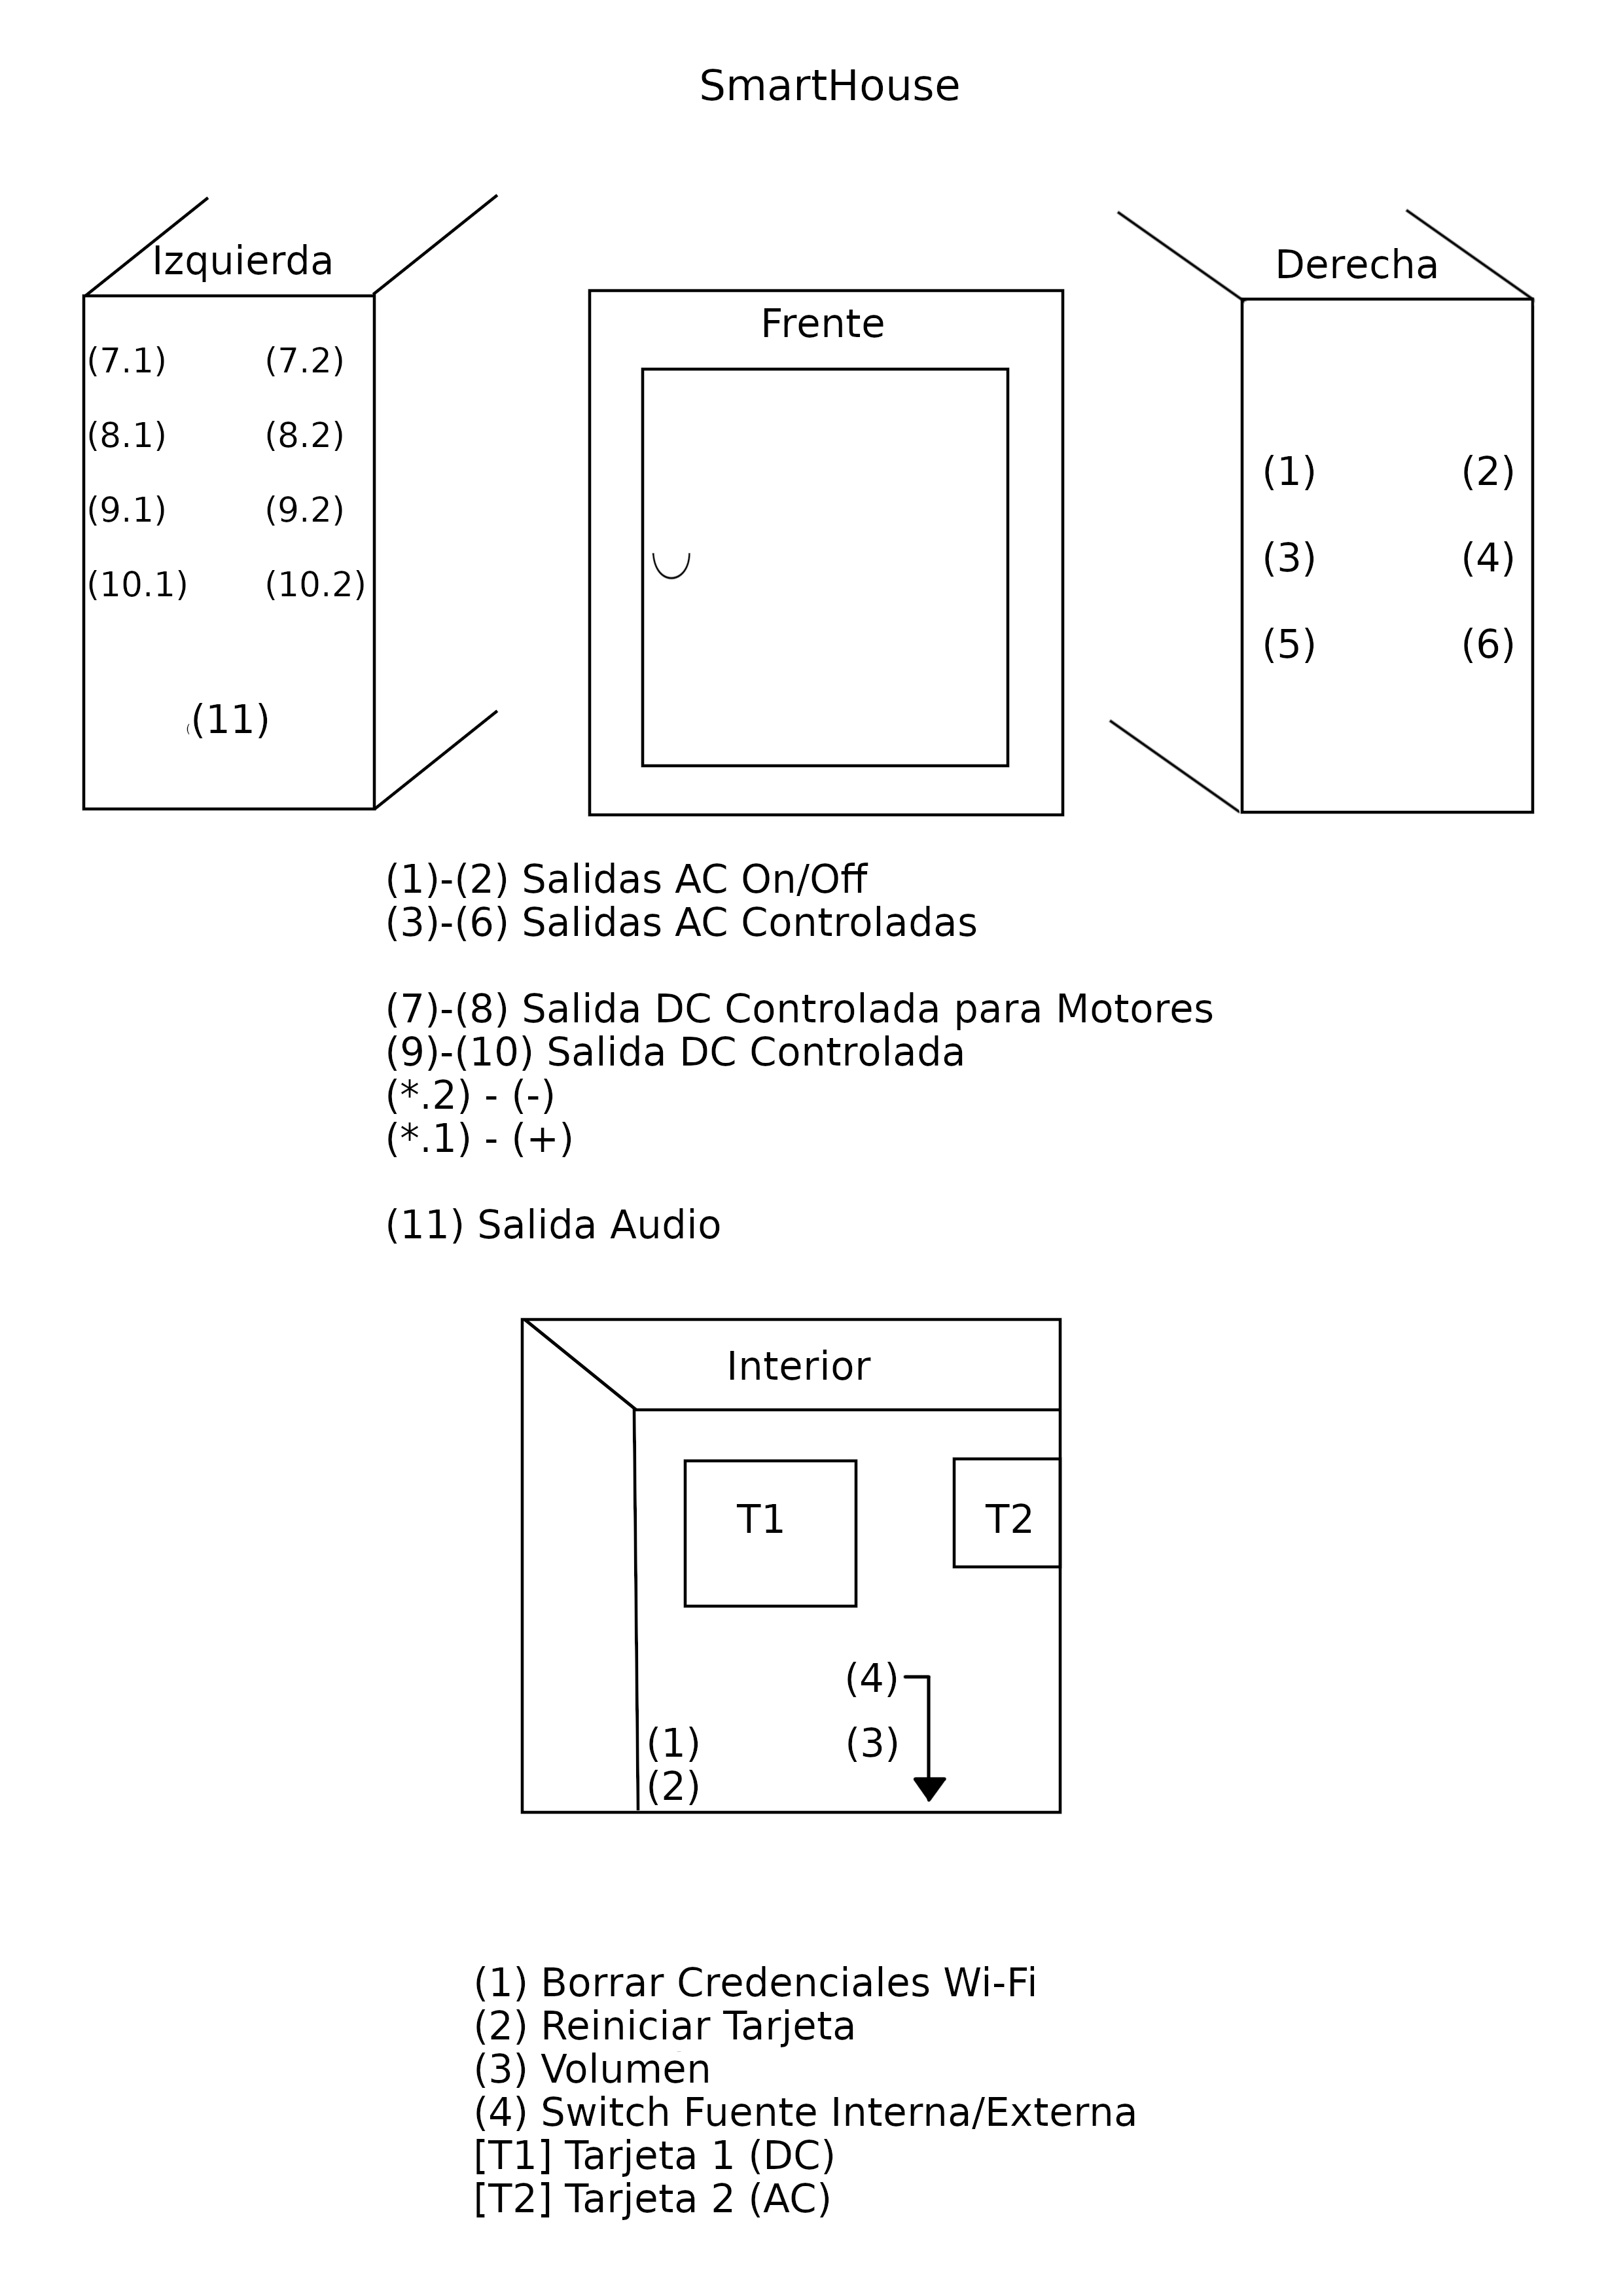
\includegraphics[width=0.7\linewidth]{Imagenes/labels}
\end{figure}

Conforme a lo mencionado anteriormente, el sistema se ha probado con cargas AC como bombillos LED entre 7W y 20W, de filamento de 100W, probando funcionalidades como el control de potencia AC por ángulo de fase, obteniendo los resultados esperados, según se observa en la figura \ref{fig:ACc}\textbf{(a)} donde la carga tiene el 100\% de la potencia y en la figura \ref{fig:ACc}\textbf{(b)} con el 20\% de esta. El voltaje de alimentación viene dado por la red eléctrica, la tarjeta simplemente conmuta el estado de la alimentación o controla la potencia entregada. \\

\begin{figure}[!t]
	\centering
	\caption{Control de potencia AC por ángulo de fase [Imagen Propia]}
	\label{fig:ACc}
	\subfigure[Potencia al 100\%]{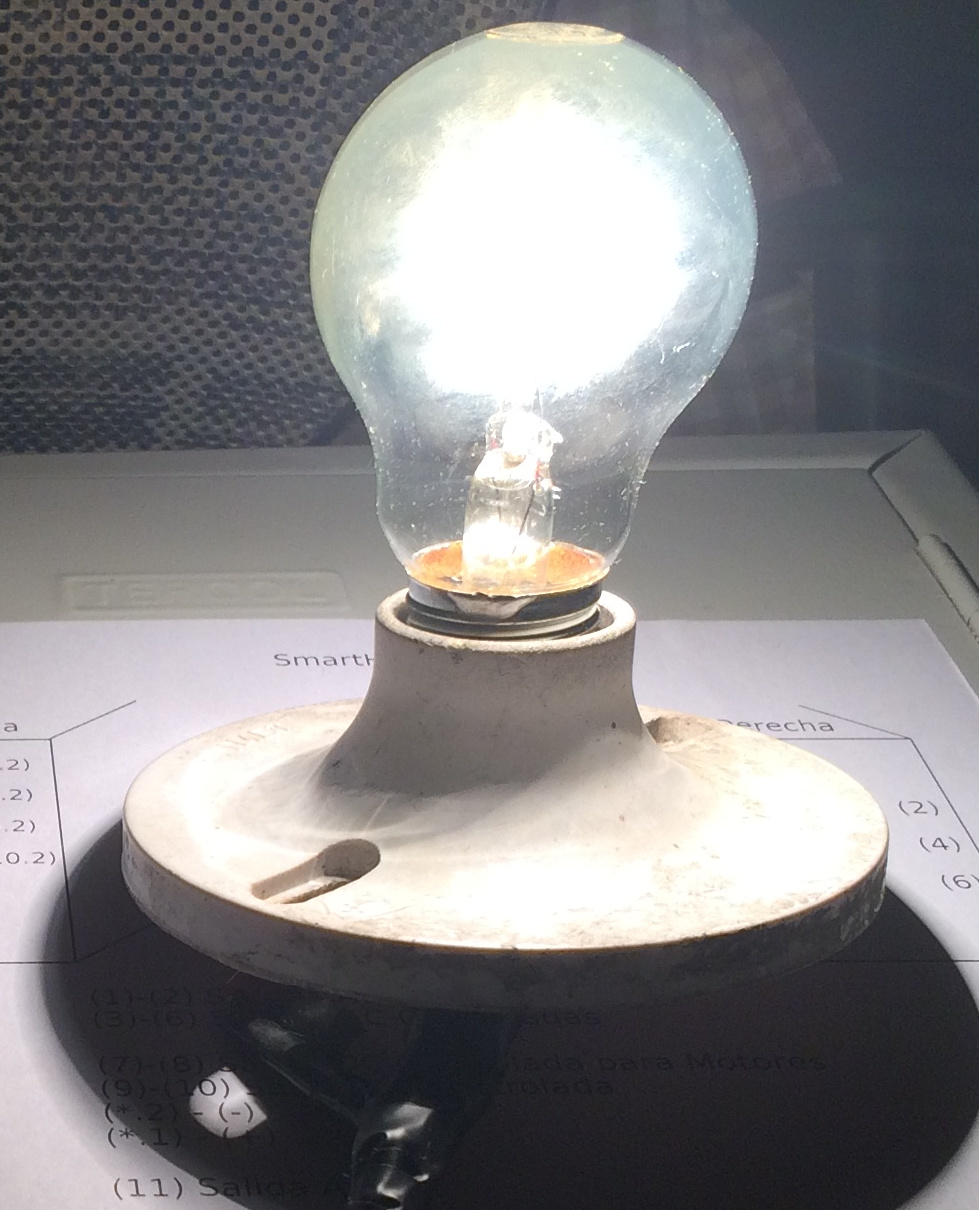
\includegraphics[width=0.45\linewidth]{Imagenes/AC1}}
	\subfigure[Potencia al 20\%]{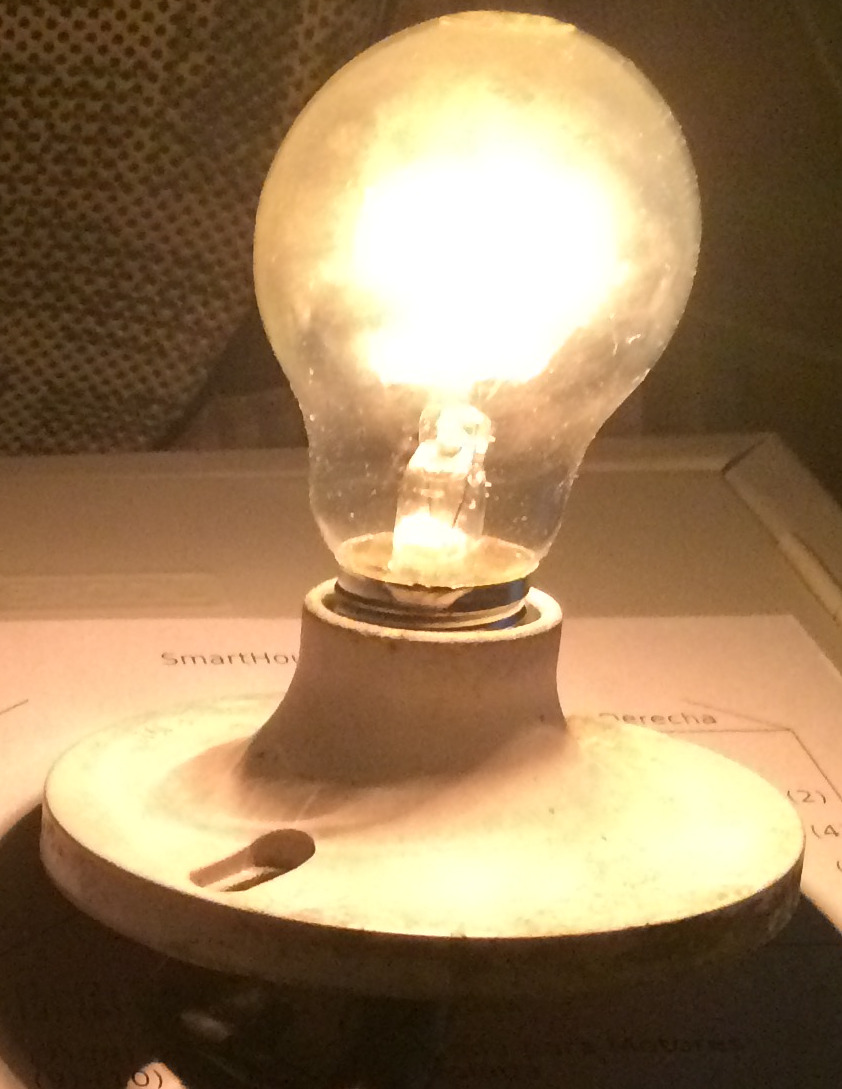
\includegraphics[width=0.43\linewidth]{Imagenes/AC0}}
\end{figure}

Para las salidas DC se realizan pruebas con un motor DC de 1W, además de una tira LED de 1W, la cual se le varia la energía entrega, como se observa en la figura \ref{fig:DCc}\textbf{(a)} la carga tiene el 100\% de la energía y en la figura \ref{fig:DCc}\textbf{(b)} solamente el 10\%. Estas cargas se alimentan con 12VDC directamente desde la fuente o convertidor AC-DC, los circuitos que se implementan simplemente conmutan el estado de encendido/apagado o por medio de PWM variar la energía entregada.\\

\begin{figure}[!t]
	\centering
	\caption{Control de Cargas DC [Imagen Propia]}
	\label{fig:DCc}
	\subfigure[Potencia al 100\%]{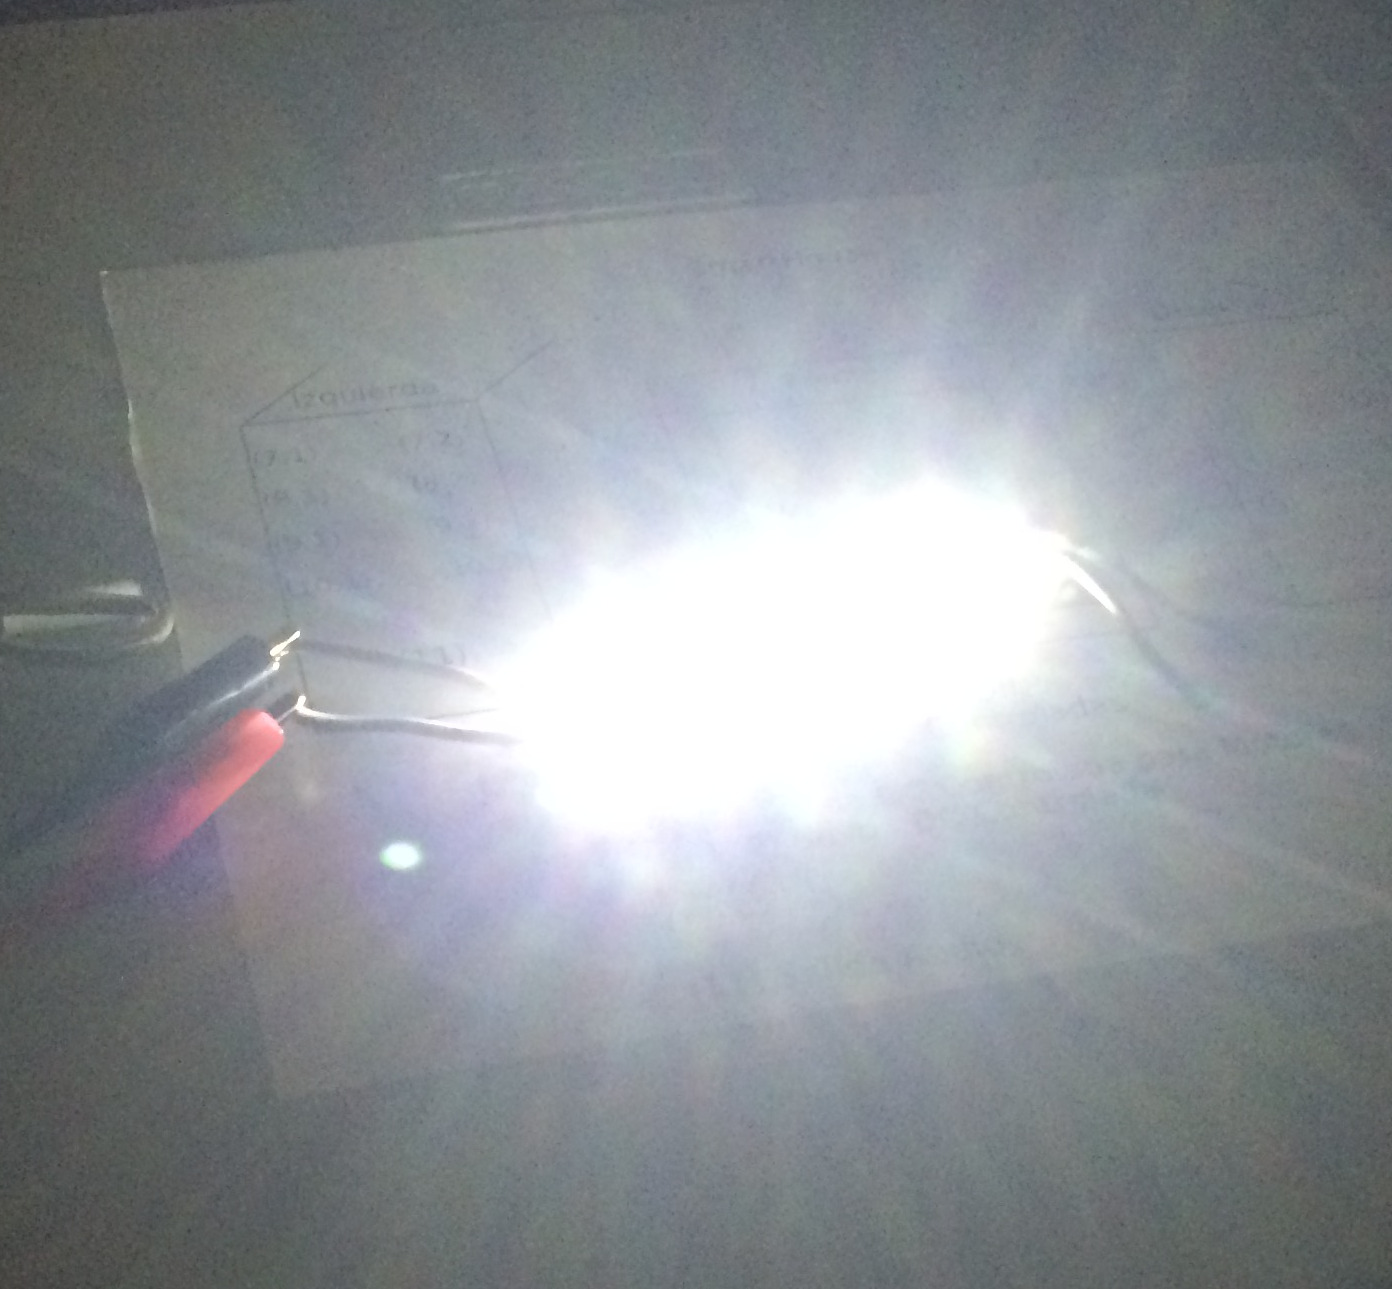
\includegraphics[width=0.45\linewidth]{Imagenes/DC1}}
	\subfigure[Potencial al 10\%]{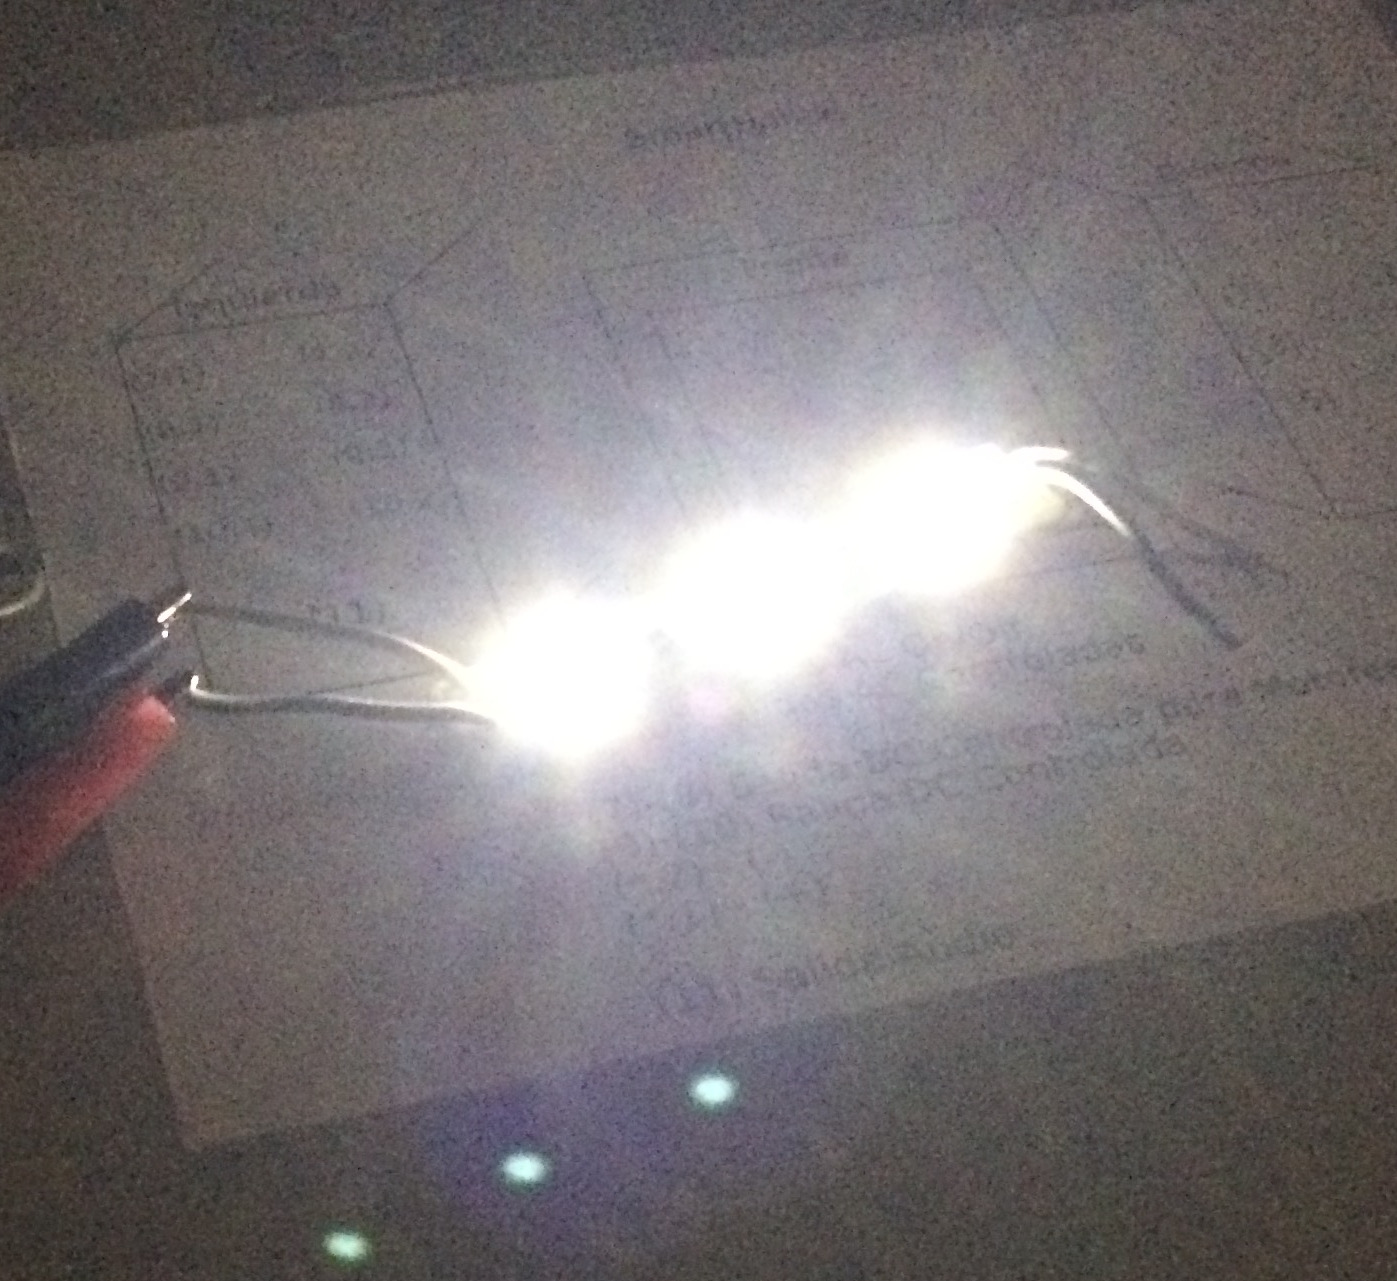
\includegraphics[width=0.455\linewidth]{Imagenes/DC0}}
\end{figure}

Se observa que el hardware quedo dividido en dos tarjetas, esto para facilitar la construcción y distribución de los diferentes elementos utilizados, si se usan componentes superficiales y se aumentan las capas de la tarjeta es posible reducir el tamaño y hasta integrarlas en una sola board. En la construcción de estas tarjetas se comprende diferentes funcionamientos en cuanto a los triac y los transistores mosfet, reforzando conocimientos que se habían adquirido.\\

\subsection{Prueba Beta Cerrada} 

Para la prueba beta se escoge un grupo de personas, las cuales interactúan directamente con la aplicación web y el prototipo de la tarjeta SmartHouse; en esta prueba se detallan diferentes ítems a evaluar, como el ingreso a la aplicación, visualización de los datos almacenados en esta y el control de los dispositivos; así, para evaluar estas características se califican de acuerdo con una escala tipo likert \cite{lik} de uno a cinco en la cual, cinco es la calificación máxima y uno la mínima.\\

La prueba se realiza a quince personas, entre los cuales algunos son estudiantes de ingería electrónica y personas ajenas a este tipo de escenarios, los resultados de la prueba se consignan en la tabla \ref{table:enc}, realizando el promedio de cada pregunta y presentando un resultado total.\\

\begin{table}
	\begin{center}
		\caption{Resultados por pregunta.}
		\label{table:enc}
		\begin{tabular}{|c|c|}
			\hline 
			\textbf{Número de la Pregunta} & \textbf{Promedio} \\ 
			\hline 
			1 & 4.5\\ 
			\hline 
			2 & 4.8\\ 
			\hline 
			3 & 4.5\\ 
			\hline 
			4 & 5.0\\ 
			\hline 
			5 & 4.9\\ 
			\hline 
			6 & 4.9\\ 
			\hline 
			7 & 4.3\\ 
			\hline 
			8 & 4.3\\ 
			\hline 
			9 & 4.8\\ 
			\hline 
			\textbf{Total} & \textbf{4.7}\\ 
			\hline 
		\end{tabular} 
	\end{center}
\end{table}

En resumen, el sistema recibe una calificación de 4.7, por lo tanto se puede decir que las funcionalidades requeridas están programadas de una manera adecuada y simple para que el usuario disponga de ellas, pero es posible mejorarlas con el objetivo de que sean mucho más intuitivas para el usuario y que no se le presenten dudas al momento de usarla. Conforme a las observaciones obtenidas durante la prueba se han modificado algunas partes del sistema, que no tienen un impacto significativo sobre los objetivos ni alcances propuestos en este trabajo.\\

Algunas características importantes resultantes de la prueba, recaen en la organización del hardware, de tal manera que sea más intuitiva la conexión y la manipulación de los botones, los cuales necesitan un posicionamiento visualmente más cómodo dentro de la caja eléctrica en la que se encuentra el sistema. Por otra parte, el manual requiere modificaciones en la explicación de algunos procesos, ya que a pesar de que este permite el uso correcto del sistema, precisa mayor detalle en procedimientos que requieren conocer aspectos como el manejo de un dispositivo inteligente o claridad adicional al usarlo por primera vez.\\

Además de esto, es importante resaltar que las interacciones de los usuarios a través de la aplicación web se realizan de manera fácil y entendible, pues los aspectos relacionados con esta y su navegación, mantienen el promedio más alto de la prueba, dejando claro que este aspecto del sistema tuvo gran éxito en cuanto a los usuarios se refiere.\\
